% Capa
\imprimircapa

% Folha de rosto
\imprimirfolhaderosto*

\begin{fichacatalografica}
	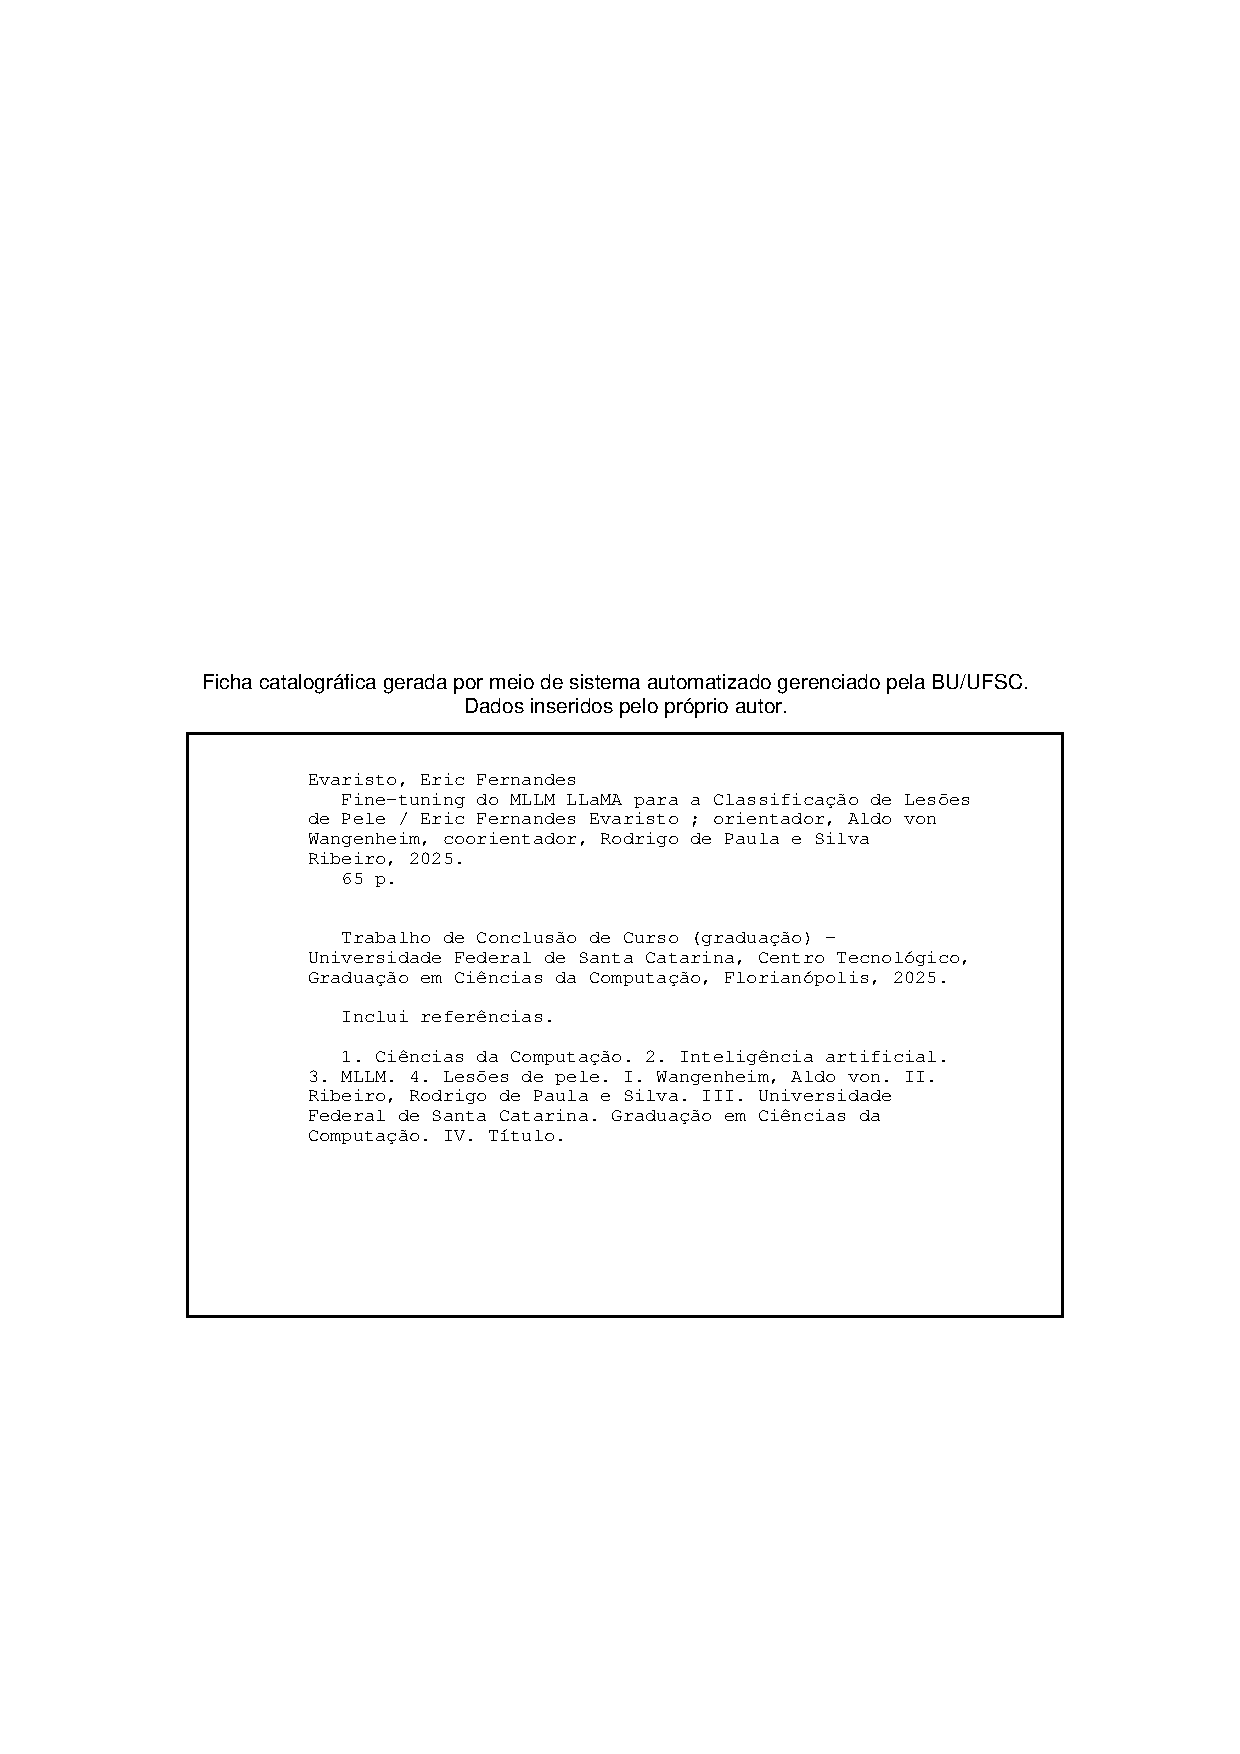
\includepdf{beforetext/Ficha_Catalografica.pdf}
\end{fichacatalografica}

% Folha de aprovação
\begin{folhadeaprovacao}
	\begin{center}
		{\imprimirautor}

		\begin{center}
			\ABNTEXchapterfont\bfseries\MakeUppercase{\imprimirtitulo}\ifnotempty{\imprimirsubtitulo}{: \imprimirsubtitulo}
		\end{center}

		\begin{minipage}{\textwidth}
			Este Trabalho de Conclusão de Curso foi julgado adequado para obtenção do Título de \imprimirformacao,
			e foi aprovado em sua forma final pelo Curso de Ciência da Computação.
		\end{minipage}%
	\end{center}

	\begin{center}
		\imprimirlocal, 15 de julho de 2025.
	\end{center}

	\assinatura{
		\textbf{\imprimircoordenador} \\
		Coordenação do Curso
	}

	\begin{center}
		\vspace{1cm}
		\textbf{Banca Examinadora:}
	\end{center}

	\vspace{1cm}
	\assinatura{
		\textbf{\imprimirorientador} \\ \imprimirorientadorRotulo
	}

	% \imprimircoorientador{
	% 	\assinatura{
	% 		\textbf{\imprimircoorientador} \\ \imprimircoorientadorRotulo \\
	% 		\imprimirinstituicao~--~\imprimirinstituicaosigla
	% 	}
	% }

	\vspace{1cm}
	\assinatura{
		\textbf{Prof. Convidado 1, Dr.} \\
		Instituição 1 -- Sigla 1
	}

	\vspace{1cm}
	\assinatura{
		\textbf{Prof. Convidado 2, Dr.} \\
		Instituição 2 -- Sigla 2
	}

	\begin{center}
		\vfill
		{
			\imprimirlocal\par
			\imprimirano\par
		}
	\end{center}
\end{folhadeaprovacao}

\begin{agradecimentos}
    ...
\end{agradecimentos}

% Resumo em português
\setlength{\absparsep}{18pt}
\begin{resumo}
	\SingleSpacing
	Lesões de pele podem ser um indicativo de diversas doenças, incluindo doenças graves como o câncer de pele. A detecção precoce dessas lesões é fundamental para o
	tratamento e cura da doença. Porém, o diagnóstico pode ser feito somente por profissionais qualificados, como dermatologistas.
	
	Uma parte do atendimento de atenção primária no Brasil é feita por \ac{ACS}. Esses profissionais estão em contato direto com a população, porém, eles não são
	qualificados para realizar a triagem de casos de lesões de pele. Considerando este cenário, uma ferramenta capaz de classificar lesões de pele e fornecer
	pré-diagnósticos pode ser útil.
	
	\acp{MLLM} possuem as capacidades necessárias para serem utilizados no desenvolvimento de uma ferramenta como esta. Estes modelos podem identificar e classificar
	lesões de pele com base em imagens e prover um pré-diagnóstico compreensível, indicando a gravidade do problema e a urgência da busca pelo atendimento médico. Além
	disso, \acp{MLLM} podem ser adaptados para tarefas especializadas através de \textit{fine-tuning}.
	
	Neste trabalho, propõe-se a adaptação do \ac{MLLM} \ac{LLaMA} 3.2 com diferentes técnicas de \textit{fine-tuning} baseadas em \ac{PEFT}, como o \ac{QLoRA} e
	\ac{LoRA}, comparando-as entre si, para classificar lesões de pele com uma acurácia aceitável.

	\textbf{Palavras-chave}: Lesões de pele. Câncer de pele. MLLM. LLaMA. PEFT. Fine tuning. QLoRA. LoRA.
\end{resumo}

% Resumo em inglês
\begin{resumo}[Abstract]
	\SingleSpacing
	\begin{otherlanguage*}{english}
		Skin lesions can indicate various diseases, including serious diseases such as skin cancer. Early detection of these lesions is fundamental for treating and
		curing the disease. However, the diagnosis can only be made by qualified professionals, such as dermatologists.

		Some primary care in Brazil is provided by \acl{ACS}, or in English, community health workers. These professionals are in direct contact with the population, but they
		are not qualified to triage cases of skin lesions. Considering this scenario, a tool capable of classifying skin lesions and providing pre-diagnosis could be
		useful.

		\aclp{MLLM} have the necessary capabilities to be used in the development of such a tool. These models can identify and classify skin lesions based on images and
		provide an understandable pre-diagnosis that indicates the severity of the problem and the urgency of seeking medical attention. In addition, \acp{MLLM} can be
		fine-tuned for specialized tasks.

		This paper proposes to adapt \ac{MLLM} \acl{LLaMA} 3.2 with different fine-tuning techniques based on \acl{PEFT}, such as \acl{QLoRA} and \acl{LoRA}, and compare
		them to classify skin lesions with acceptable accuracy.

		\textbf{Keywords}: Skin lesions. Skin cancer. MLLM. LLaMA. PEFT. Fine tuning. QLoRA. LoRA.
	\end{otherlanguage*}
\end{resumo}

{
\hypersetup{hidelinks}

% Lista de imagens
\pdfbookmark[0]{\listfigurename}{lof}
\listoffigures

% Lista de siglas
\imprimirlistadesiglas

% Sumário
\pdfbookmark[0]{\contentsname}{toc}
\tableofcontents*
\cleardoublepage
}
